\documentclass[11pt,a4paper]{article}
\usepackage[a4paper,margin=2.35cm]{geometry}
\usepackage{fontspec}
\setmainfont{Times New Roman}
\usepackage{amsmath,amssymb}
\usepackage{graphicx}
\usepackage{booktabs}
\usepackage{caption}
\usepackage{placeins}
\captionsetup{font=small,labelfont=bf}
\usepackage[colorlinks=true,linkcolor=black,citecolor=black,urlcolor=blue]{hyperref}
\setlength{\parindent}{0pt}
\setlength{\parskip}{0.28em}
\setlength{\emergencystretch}{1em}

\begin{document}
\begin{center}
{\LARGE\bfseries BroadcastGuard: A Controlled Study of Low-Exponent RSA Broadcast Recovery and Authenticated Multi-Recipient Sharing\par}
\vspace{0.55em}
{\small
\begin{tabular}{cc}
Nguyễn Tiến Dũng (23BA14068) & Vũ Minh Châu (23BA14028) \\
Nguyễn Minh Hiếu (23BA14105) & Lê Đức Anh (23BA14005) \\
Hoàng Lê Anh Đức (23BA14057) & Lê Vân (2411065) \\
Phạm Duy Đức Tâm (23BA14253) & \\
\end{tabular}\par}
\vspace{0.25em}
{\small University of Science and Technology of Hanoi (USTH)}
\end{center}
\vspace{-0.55em}

\begin{abstract}
Textbook RSA with a small public exponent can expose a message sent unchanged to several recipients. BroadcastGuard connects the exact integer condition for this recovery to controlled experiments and to a safer multi-recipient design. Across 20 independent RSA key sets, all 560 subset trials agreed with the CRT-and-cube-root prediction; two 96-byte inputs had different recovery thresholds because their integer values differed. In 60 same-key comparisons, the tested procedure recovered textbook plaintext 60 times and OAEP plaintext zero times, while legitimate OAEP decryption succeeded throughout. Hybrid file experiments separate encryption and key wrapping from JSON/Base64 serialization; the latter dominated measured 1 MiB workflows on one machine. These observations support an educational analysis, not a new cryptographic primitive or a universal security proof.
\end{abstract}

\section{Introduction and motivation}
RSA represents plaintext as an integer and applies public modular exponentiation~\cite{rivest1978method}. Without randomized encoding, sending one integer to different recipients with a small exponent creates a public algebraic relation. Håstad studied broader low-degree, multi-modulus vulnerabilities~\cite{hastad1988solving}; our fixed-message case has a shorter CRT argument. We ask exactly \emph{when} that computation returns the original bytes and what a same-key padding comparison establishes.

BroadcastGuard combines a seven-subset conditions analyzer, a same-key textbook/OAEP comparison, authenticated hybrid file sharing, and reproducible evaluation. RSA, CRT, OAEP and GCM are established. \href{https://github.com/Dung092005/Crypto-project}{Source and evidence} and an \href{https://broadcastguard-crypto.streamlit.app/}{interactive demonstration} are available; the interface is a teaching aid, not independent security evidence.

\section{Background and attack model}
Eve observes public pairs $(n_i,e)$ and ciphertexts $c_i$, but no private keys. In the attack experiment, the same byte string is converted to a nonnegative integer $M$ and encrypted without padding under distinct pairwise-coprime RSA moduli, with $e=3$ and $M<n_i$. For any nonempty observed subset $S$,
\begin{equation}\label{eq:crt}
 c_i=M^3\bmod n_i,\qquad N_S=\prod_{i\in S}n_i,\qquad X=\operatorname{CRT}(\{c_i,n_i\}_{i\in S})=M^3\bmod N_S.
\end{equation}
CRT returns the unique $X\in[0,N_S)$. Thus $M^3<N_S$ implies $X=M^3$, whose exact integer cube root is $M$. Conversely, recovery of $M$ by this particular nonnegative CRT-and-root procedure requires that inequality. An exact cube root of $X$ alone may be a \emph{different} integer; only the experimenter compares the candidate with the original $M$. Eve's algorithm receives no ground truth. The original byte length is retained separately because leading zero bytes disappear in integer conversion.

OAEP applies randomized encoding before RSA exponentiation~\cite{bellare1995optimal,moriarty2016pkcs1}. Its ciphertexts do not encode a common unpadded $M^3$ relation across recipients. RFC~8017 specifies RSAES-OAEP and the limit $m_{\rm Len}\leq k-2h_{\rm Len}-2$; RSA-2048 with SHA-256 therefore accepts at most 190 message bytes~\cite{moriarty2016pkcs1}. Our comparison applies the \emph{same} CRT-and-root procedure to OAEP ciphertext integers to test its observed outcome, without treating them as textbook ciphertexts.

\section{System design and experimental method}
The educational attack builder generates three RSA-2048/e=3 keypairs for Alice, Bob and Charlie. A public-only attacker combines any selected observations using CRT and an integer-only cube root; a separate evaluator checks the original message and the inequality in Eq.~\eqref{eq:crt}. The analyzer enumerates all seven nonempty recipient subsets. In E1, 20 independently generated key-set blocks each test four messages on the \emph{same} three moduli: \texttt{B} repeated 1, 96 or 180 times, and 95 zero bytes followed by \texttt{0x02}. E2 uses the same key set and plaintext within each paired textbook/OAEP trial; OAEP uses SHA-256, MGF1(SHA-256) and the empty label. The three message samples give 60 paired observations in 20 key-set blocks, not 60 independent key sets.

Secure Sharing uses a separate RSA-2048/e=65537 configuration. For each file, it generates a fresh 256-bit AES key and 96-bit GCM nonce, encrypts file bytes \emph{once} with AES-GCM, and RSA-OAEP-wraps that key independently for each recipient. A compact, canonical JSON header (filename, size, nonce, algorithm identifiers, recipient IDs, public-key fingerprints and wrapped keys) is GCM associated authenticated data; the ciphertext and 16-byte tag are stored as Base64 in a versioned JSON package. A matching private key unwraps the AES key; authenticated decryption returns bytes only after validation. GCM authenticates ciphertext and AAD under the key, not the sender's identity~\cite{dworkin2007gcm}.

E3 times nine combinations of 10\,KiB, 100\,KiB and 1\,MiB files with one, three or five recipients, using 20 measured repetitions and two warmups per configuration. Prepared RSA keys are reused for routine workflow timing; independent key generation is timed separately. \texttt{perf\_counter\_ns} intervals distinguish encrypt+wrap, JSON/Base64 serialization, their sum, and decryption for the first valid recipient. All decrypted files are compared byte-for-byte. E4 checks one valid package and ten selected invalid, mismatched or modified cases. The archived \href{https://github.com/Dung092005/Crypto-project/tree/main/docs/evidence/official-20261106T083221Z-3bbf57cc}{official run} records its manifest, source commit, raw CSVs and validation status; no observations were discarded.

\section{Results and analysis}
\subsection{The integer boundary, not byte count}
Figure~\ref{fig:e1} reports all seven subset outcomes. Across $20\times4\times7=560$ trials, the inequality in Eq.~\eqref{eq:crt} matched the evaluator's recovery result in every row. The minimum successful interception count was one, two, three and one for the four declared samples, respectively. Both 96-byte inputs have identical storage length, yet \texttt{B}$^{96}$ is a 767-bit integer while the leading-zero sample represents the integer 2. Consequently, a single ciphertext suffices for the latter, whereas any two of the three suffice for the former. This verifies the numerical bound for these controlled inputs; it does not imply that all 96-byte messages share one threshold.

\begin{figure}[!ht]
\centering
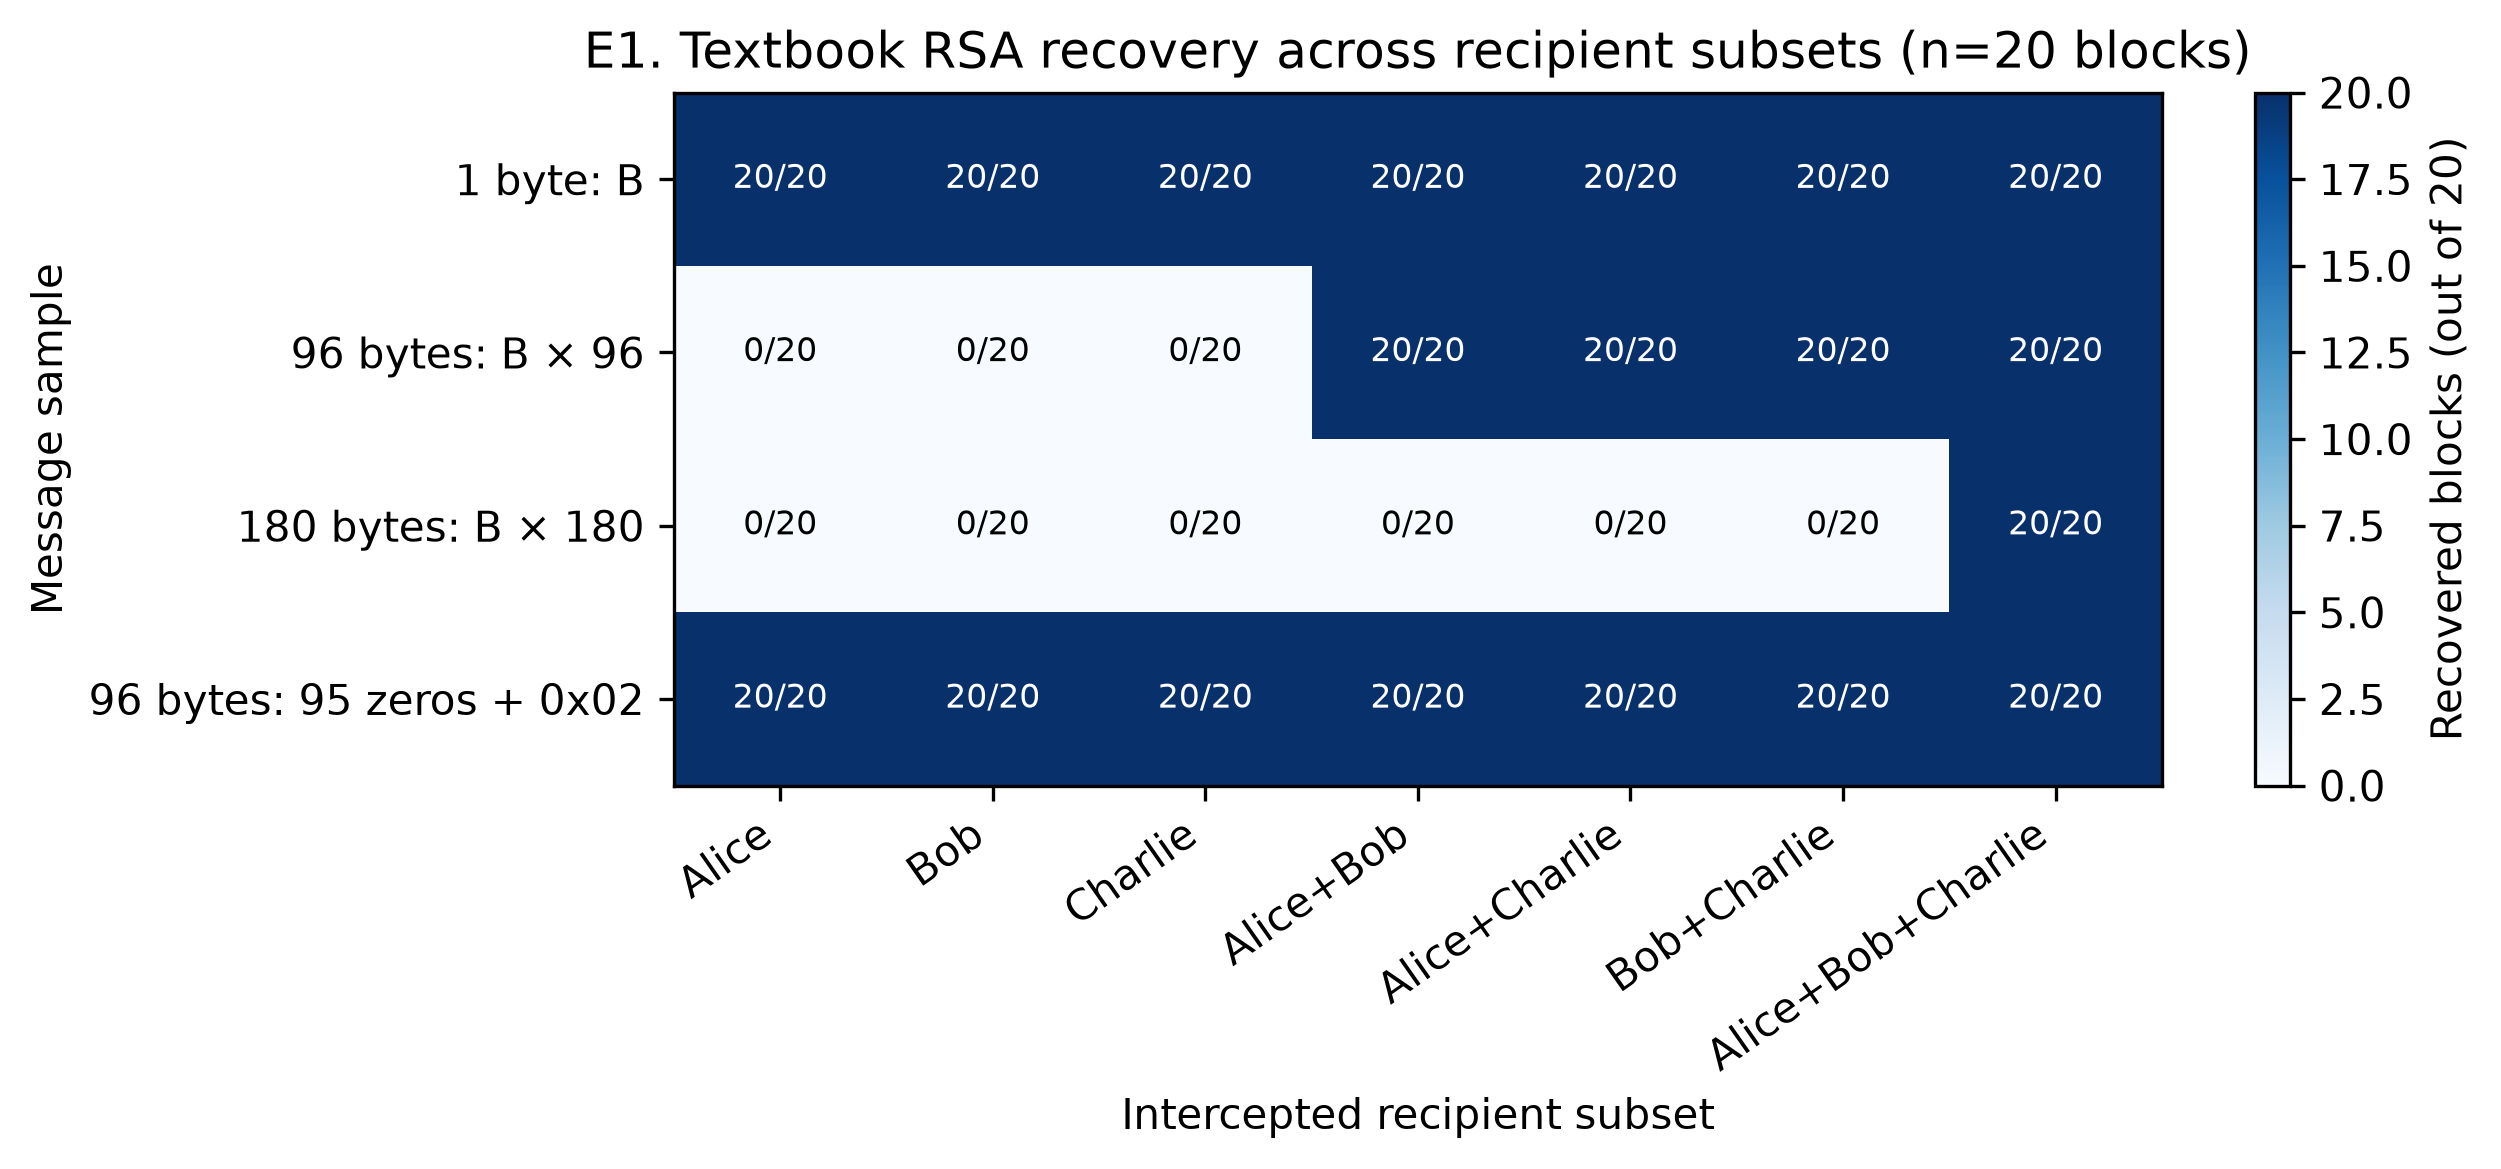
\includegraphics[width=\linewidth]{../docs/analysis/figures/figure_1_e1_recovery_matrix.png}
\caption{Textbook RSA original-plaintext recovery for four fixed messages and all seven intercepted subsets, across 20 independent RSA-2048/e=3 key-set blocks. Cells show successful blocks out of 20. The two 96-byte rows differ in integer value despite identical byte count.}
\label{fig:e1}
\end{figure}

\subsection{Paired padding comparison}
Table~\ref{tab:e2} uses identical plaintext, three recipients, RSA keypairs, exponent and attack procedure within each comparison; only the encryption scheme changes. Textbook encryption repeats the same ciphertext for the same key and message; OAEP's randomized encoding produced distinct repeated ciphertexts in all 60 checks. The tested CRT-and-root computation recovered no original OAEP plaintext, while every legitimate recipient decrypted correctly. These 60 observations are clustered in 20 independent key-set blocks. Their result does not constitute a formal proof of OAEP security or a test of every attack.

\begin{table}[!ht]
\centering
\caption{E2 outcomes across 60 paired comparisons in 20 RSA key-set blocks. Recovery means equality with the original plaintext, checked by the evaluator; decryption is a distinct legitimate-recipient operation.}
\label{tab:e2}
\begin{tabular}{@{}llr@{}}
\toprule
Scheme & Procedure/outcome & Correct / trials\\
\midrule
Textbook RSA & Eve's CRT-and-root recovery & 60/60\\
RSA-OAEP & Eve's same procedure & 0/60\\
RSA-OAEP & Legitimate decryption & 60/60\\
\bottomrule
\end{tabular}
\end{table}
\FloatBarrier

\subsection{Hybrid cost and authenticated failure}
Figure~\ref{fig:e3} separates application packaging from cryptographic work. For a 1\,MiB file and one recipient, the raw means were 0.479550\,ms for encrypt+wrap and 7.232030\,ms for serialization; their 7.711580\,ms sum excludes RSA key generation. Serialization accounted for 93.78\% of that measured mean on this Windows system. The three 1\,MiB total means were not monotone in recipient count, so small differences should not be interpreted as an algorithmic speed advantage; the recorded distributions and scheduling variability matter. The decryption interval measures only one valid recipient.

\begin{figure}[!ht]
\centering
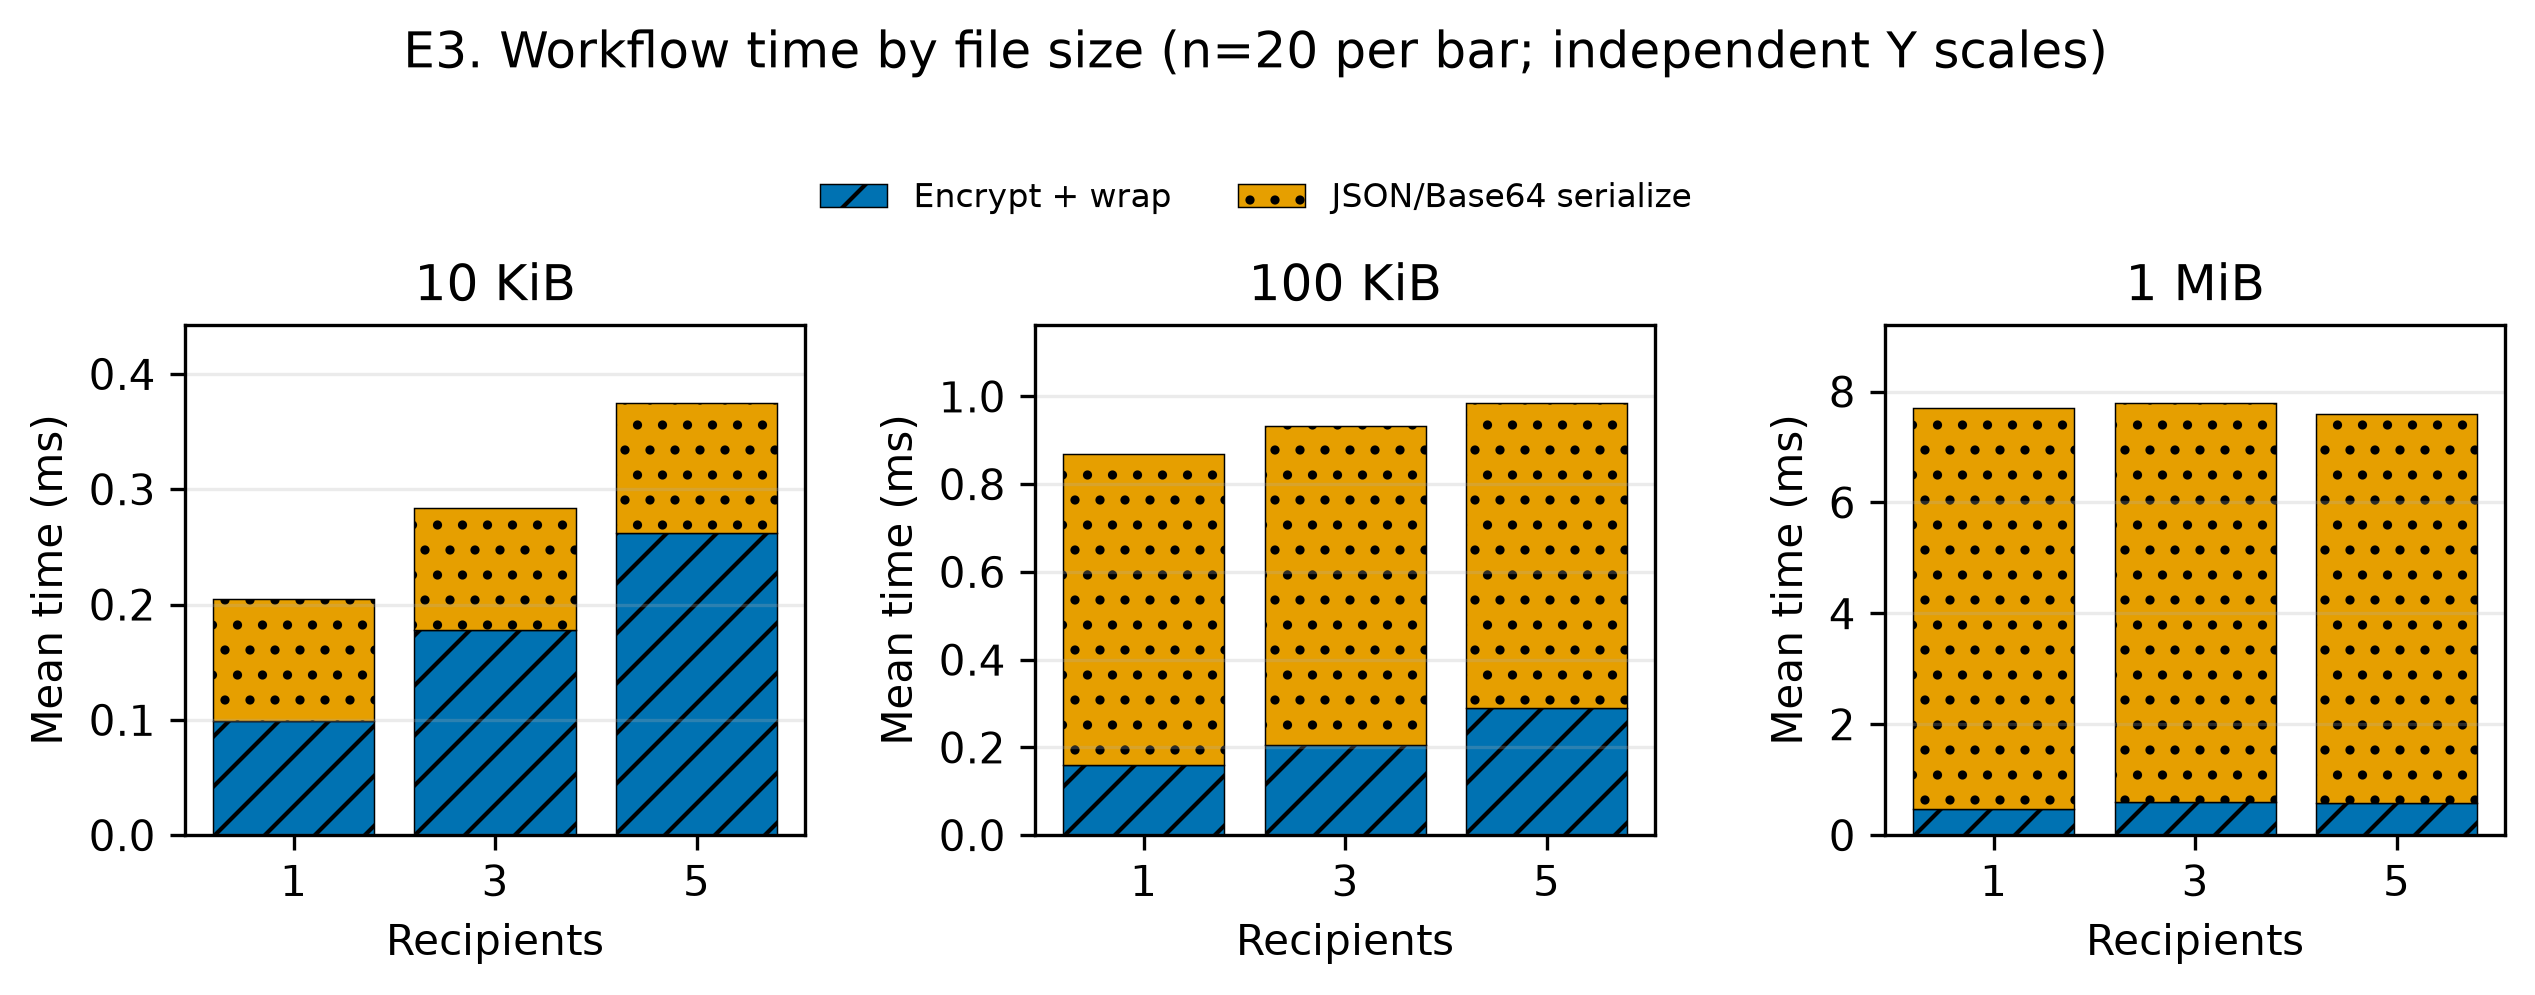
\includegraphics[width=\linewidth]{../docs/analysis/figures/figure_3_e3_timing_decomposition.png}
\caption{Mean E3 workflow components in milliseconds, 20 timed repetitions per file-size/recipient configuration with prepared keys. Each file-size panel has an independent, zero-based Y-axis scale. Total encryption is encrypt+wrap plus JSON/Base64 serialization; key generation is measured separately.}
\label{fig:e3}
\end{figure}

The serialized package size is structurally
\begin{equation}\label{eq:size}
P(L,r)=4\left\lceil\frac{L+16}{3}\right\rceil+H(L,r,f,\mathcal I),
\end{equation}
where $L$ is plaintext bytes, $r$ is recipient count, 16 is the GCM tag length, and $H$ includes JSON structure, filename $f$, decimal size, nonce, IDs $\mathcal I$, fingerprints and one Base64-encoded 256-byte RSA wrapped key per recipient. For the fixed E3 filenames and IDs, this exact accounting matched every observed serialized size; it is not a fitted law for arbitrary metadata. At 1\,MiB the observed relative overhead ranged from 33.40\% (one recipient) to 33.58\% (five), mostly reflecting Base64's approximate one-third expansion rather than the GCM tag alone.

All 11 E4 correctness cases matched expected outcomes: the valid case returned original bytes, and ten malformed, mismatched or modified cases returned no plaintext. Rejection may arise from structure checks, a wrong recipient/key, OAEP failure or GCM authentication; it does not by itself identify malicious tampering.

\section{Limitations and discussion}
E1 verifies a known elementary condition; Håstad considered broader low-degree modular systems. E2's zero OAEP recoveries concern one procedure and sample, not all attacks. E3's 20 wall-clock timings per configuration come from one Windows computer; scheduling and interpreter effects limit generalization, and decryption covers only the first recipient. E4 is a selected checklist, not an attack population. Sharing assumes authenticated recipient public keys; fingerprints alone do not establish identity. Filename and recipient metadata remain visible. The implementation lacks sender authentication, replay protection, PKI and persistent key management.

\section{Conclusion}
The bound $M^3<N_S$ predicted every E1 subset outcome and explains why byte count alone misleads. In the paired comparison, the tested CRT-and-root method did not recover OAEP plaintext, while intended recipients decrypted. For hybrid files, JSON/Base64 serialization dominated the observed 1\,MiB workflow. BroadcastGuard contributes controlled integration, auditable implementation and explicit evidence limits, rather than a new cryptographic algorithm.

\small
\bibliographystyle{IEEEtran}
\bibliography{../research/broadcastguard/REFERENCES}
\end{document}
